% !TEX encoding = UTF-8 Unicode
%!TEX root = main.tex
% !TEX spellcheck = en-US
%%=========================================


%%%%%%%%%%%%%%%%%%%%%%%%%%%%%%%%%%%%%%%%%%%%%%%%%%%%%%%%%%%%%%%%%%%%%%%%%%%%%%%%%%%%%%%%%%%%%%
\chapter{Background}
\label{ch:background}

In this chapter a more in\hyp{}depth explanation of the different topics introduced in the introduction chapter is presented. These topics cover the required background knowledge for the project, which plays a important role in determining on what kind of development tool is to be implemented, how it is to be implemented, as well as showing what already exists of current solutions and tools.

Each topic is presented on its own, and how it relates to the paper.


%%%%%%%%%%%%%%%%%%%%%%%%%%%%%%%%%%%%%%%%%%%%%%%%%%%%%%%%%%%%%%%%%%%%%%%%%%%%%%%%%%%%%%%%%%%%%%%
\section{Concurrency vs. Parallelism}
\label{sec:concurrency_vs_parallelism}

The notion of parallelism and concurrency in programs spawns from the limitations of sequential programs. All programming languages have different ways to express the structure and control flow of a program, but in the end all programs are transformed to machine code which the processor executes \textit{sequentially}. That means for a single processor, only one instruction is executed at a time\footnote{This implies the processor is single-core}. Concurrency however defines a program into multiple independent sequential programs, which in turn runs each sequential program in interleaving time periods. Even though only one instruction is executed at a time, this gives the impression that multiple sequential programs are advancing at the same time.

Parallelism in this sense refers to multiple programs running on multiple processors in parallel. This might look familiar to how concurrency is described, but it is important to not confuse these two terms together. Concurrency only serves as an abstraction for parallelism in a program, allowing the programmer to pretend multiple sequential programs are executed in parallel. This abstraction would be valid for both single and multi\hyp{}core, while parallelism describes a condition which only happens on multi\hyp{}core architectures. A more thorough and complete definition of concurrency and parallelism is described in \citet{benari2006}.

Concurrency and parallelism forms the very core of this project. Section \ref{sec:csp} explains what CSP is, which forms its basis on concurrency. Understanding the underlying concepts of concurrency is important to understand what CSP entails.


%%%%%%%%%%%%%%%%%%%%%%%%%%%%%%%%%%%%%%%%%%%%%%%%%%%%%%%%%%%%%%%%%%%%%%%%%%%%%%%%%%%%%%%%%%%%%%
\section{Threading Models}
\label{sec:threading_models}

As concurrency is a superb tool for programmers to abstract parallelism in their program, the implementation details of this is equally as important for this project. There are different ways to implement this, but almost all concurrency models implement some sort of a threading mechanism. When talking about threading mechanisms on \textit{Operating Systems} (OS), one usually talks about two kinds of threads: user- and kernel-threads. As the names may imply, these threads operate in either user- or kernel-space. Three main models explains the different combinations of the two threads: user-, kernel-, and hybrid-threading models. \citet{c++csp2} goes further into details on these models, and short summary is presented below from said article.

In short, the user\hyp{}threading model implements a cooperative scheduled threading in user\hyp{}space, and is called a \texttt{M:1} threading model. This model is running \texttt{M} user-threads on a single kernel\hyp{}thread, where everything from scheduling and context switching is happening unbeknownst to the kernel\hyp{}thread. This threading mechanism is not visible to the OS, and avoids the overhead related to context switches in kernel-threads. However, blocking calls are a challenge, as a single blocking call will block all user-threads.

Kernel\hyp{}threading model is often directly supported in OS kernels, and is called a \texttt{1:1} threading model. Each kernel\hyp{}thread is scheduled by the OS onto the the systems processors, which is often implemented as preemptive scheduling. Due to kernel\hyp{}threads residing in kernel\hyp{}space, context switches has a much larger overhead than user\hyp{}threading. Blocking calls are however not a problem. 

Hybrid-threading model combines the two models, and is called a \texttt{M:N} threading model. This model is running multiple kernel\hyp{}threads, with each kernel-thread running multiple user\hyp{}threads. Blocking calls is still a problem, but can be mitigated through dispatching a single kernel\hyp{}thread for the block user\hyp{}thread, and continue the rest of the scheduling on a new kernel\hyp{}thread. 


%%%%%%%%%%%%%%%%%%%%%%%%%%%%%%%%%%%%%%%%%%%%%%%%%%%%%%%%%%%%%%%%%%%%%%%%%%%%%%%%%%%%%%%%%%%%%%%%%%%
\section{Memory Layout of C Programs}
\label{sec:memory_layout_c}

\FloatBarrier

The C programming language defines a memory layout of its programs. A total of 5 sections defines the memory layout.

\begin{enumerate}[topsep=0em,itemsep=-1em,partopsep=0.5em,parsep=1em]
    \item Text segment
    \item Initialized data segment
    \item Uninitialized data segment
    \item Stack
    \item Heap
\end{enumerate}

The text segment contains the executable code of instructions. The initialized data segment contains global and static variables that are initialized by the programmer. The uninitialized data segment contains all zero initialized or non\hyp{}initialized variables and data. The stack contains the program stack and stack frames, while the heap contains dynamic memory. The stack grows downwards, from higher to lower address, opposed to the heap which grows upwards, from lower to higher address. 

The unmapped segment is a precursor to the stack, containing command-line arguments and environment variables sent as program arguments. 

See Figure \ref{fig:c_memory_layout} for outline of the memory layout.

\begin{figure}[h!]
    \centering
    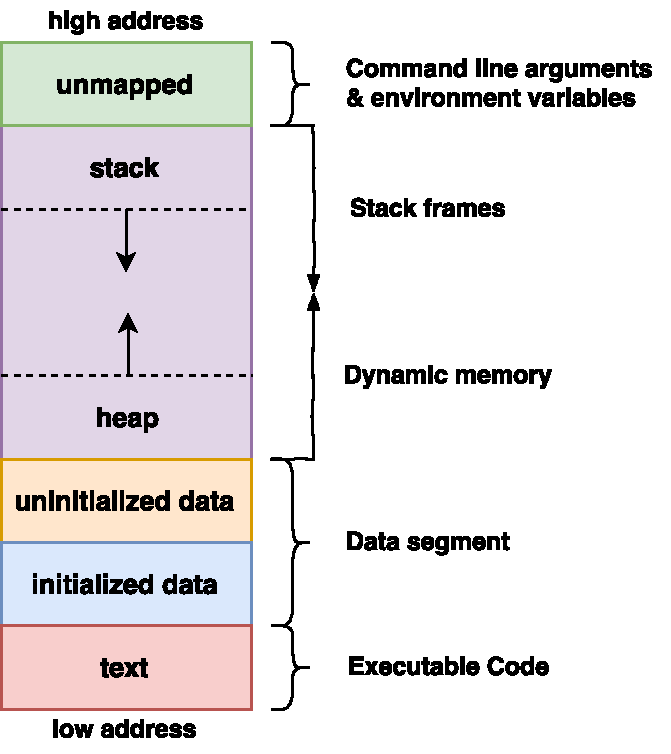
\includegraphics[width=0.5\linewidth]{fig/c_memory_layout}
    \caption{Memory layout of a C program}
    \label{fig:c_memory_layout}
\end{figure}

\FloatBarrier


%%%%%%%%%%%%%%%%%%%%%%%%%%%%%%%%%%%%%%%%%%%%%%%%%%%%%%%%%%%%%%%%%%%%%%%%%%%%%%%%%%%%%%%%%%%%%%%%%
\section{Stackful Coroutines}
\label{sec:stackful_coroutines}

Coroutines are a generalized subroutines within a program, used for non-preemptive multitasking. This allows a single\hyp{}threaded program to suspend and resume multiple executions, through predetermined scheduling points. There exists two types of coroutine implementations: stackful and stackless. As the name implies, stackful coroutines each has its own stack. While for stackless coroutines, the main stack frame is used by all coroutines.

Resuming and suspending stackful coroutines involves storing and swapping contexts of coroutines. Each coroutine has a context which represents the execution state of a coroutine at a given time. This execution state can be seen as a snapshot of the processor registers at a given place in the code execution. Suspending a coroutine is a matter of storing the current execution state in memory, and replace the execution state with another coroutine. Lastly, the program counter is replaced with the resuming coroutine. This effectively suspends the initial coroutine, and resumes the other. 

Knowing what to store in execution states requires knowledge of the processor state, which is architecture dependent. This is why coroutine implementations often causes portability issues. The solution to this is looking at the calling convention for System V \textit{Application Binary Interface} (ABI) \citep{systemvabi}, which is the convention almost all UNIX\hyp{}like architectures follow. 

Calling conventions describes, on a low\hyp{}level, how subroutines receive parameters from their caller and how they return their result. This usually describes on register level which registers must be preserved by the callee, and which must not. Knowing this, a context structure and a context switching procedure can be outlined. 

The context structure should contain the preserved registers specified by the calling convention and the program counter for a given coroutine. The context switch procedure must be a function call. This means all volatile variables remaining in non\hyp{}preserved registers will be pushed to the stack before calling the procedure. Then, in the procedure, all preserved registers are stored in the context structure, along with the program counter. When resuming, the preserved registers are loaded from the context structure and lastly sets its own program counter. This will cause a jump to the other coroutine context, which resumes as if the context switching procedure call returned. 


%%%%%%%%%%%%%%%%%%%%%%%%%%%%%%%%%%%%%%%%%%%%%%%%%%%%%%%%%%%%%%%%%%%%%%%%%%%%%%%%%%%%%%%%%%%%%%%%
\section{Communicating Sequential Processes}
\label{sec:csp}

First introduced by Tony Hoare in 1978 \citep{csp}, Communicating Sequential Programming (CSP) aimed to make concurrency and parallelism a much more convenient tool for programmers. Even though CSP in itself is a mathematical formal language, the concepts and structuring it introduces is very applicable as a programming model. The core concept of CSP is a composition of concurrent sequential processes, which strictly communicate by message passing via channels.

Despite CSP being a great model for describing concurrent systems, it has not gained much mainstream traction within programming communities and industries. As detailed in \citet{benari2006}, concurrent programming introduces new challenges such as race conditions, deadlocks and fairness. These challenges can for many programmers be a hurdle to create correct concurrent programs, shown in \citet{ousterhour1996}. As a result of this they might end up opting in for other simpler programming models, and in turn miss out of CSP. 

This does not mean however that there does not exists CSP implementations. These implementations range from programming languages which implements the CSP model (Section \ref{subsec:csp_prog_lang}), CSP libraries for more mainstream non-CSP programming languages (Section \ref{subsec:csp_prog_lib}), and CSP language compilers (Section \ref{subsec:csp_comp_runtime}).

The CSP implementations range in varying popularity and use, and below is a summary of the most notable entries which relates to this project presented.


%%%%%%%%%%%%%%%%%%%%%%%%%%%%%%%%%%
\subsection{Programming Languages}
\label{subsec:csp_prog_lang}

Multiple programming languages implementing the CSP models in varying degree exists. Probably the most notable and truest implementation of the CSP model is occam. Other languages such as XC and Go is heavily influenced by the CSP model and occam. There exists other CSP languages such as Limbo \citep{limbo}, Joyce \citep{joyce}, and SuperPascal \citep{superpascal}, however occam, XC and Go seems to be the most influential and used languages to date\footnote{This is a highly subjective view, based on the popularity and relevance in the industry}. 


%%%%%%%%%%%%%%%%%%%%%
\subsubsection{occam}
\label{sssec:occam}

Occam is a concurrent programming language which builds upon the CSP model. It was created by INMOS \citep{occam} and first appeared in 1983. Occam was initially developed as the native programming language for the Transputer, their microprocessor architecture highly specialized for real-time parallel computing \citep{transputer}. 

Occam was initially only developed for the Transputer, making it hardware locked and inaccessible for everyone not using the Transputer. However, occam proved to be quite expressive and useful for concurrent programming, which spurred multiple ports and compilers of occam to other open architectures. Sadly, occam never received the appropriate recognition it deserved, and instead got its place in a niche market of real\hyp{}time parallel computing with its highly specialized microprocessor Transputer. 

All occam programs consists of processes. These processes can either be expressed as a single statements, or as a collection of multiple statements. What is very different in occam compared to other languages, is the native support for parallelism. The \texttt{PAR} keyword specifies a parallel execution between one\hyp{}or\hyp{}more processes. There is an equivalent keyword for sequential execution, called \texttt{SEQ}. All statements in occam must be explicitly specified if they are executed in sequence or parallel. 

\noindent\begin{minipage}{0.45\textwidth}
\begin{lstlisting}[style={CustomC},frame={},numbers={none},xleftmargin={4em}]
PAR
  p()
  q()
  z()
\end{lstlisting}
\end{minipage}
\begin{minipage}{0.45\textwidth}
\begin{lstlisting}[style={CustomC},frame={},numbers={none},xleftmargin={4em}]
SEQ
  x := 10
  x := x + 1
  y := x * x
\end{lstlisting}
\end{minipage}

Processes can be defined with the \texttt{PROC} keyword. The process can have zero\hyp{}or\hyp{}more arguments. 

\noindent\begin{minipage}{\textwidth}
\begin{lstlisting}[style={CustomC},frame={},numbers={none},xleftmargin={4em}]
PROC system()
  SEQ
    i := 1
    i := i + 1
:   
\end{lstlisting}
\end{minipage}

Processes are not allowed to share memory. All communication between processes is done through channels. Channels in occam are unbuffered and synchronized, which means both a sender and a receiver must be present on a channel to complete the transfer of data. Channels are also typed. Occam also requires disjointness on channels, meaning only one unique process can be a sender and a receiver on a given channel. In occam, the operator ``\texttt{!}'' is used to send on a channel, and ``\texttt{?}'' to receive on a channel.

\noindent\begin{minipage}{\textwidth}
\begin{lstlisting}[style={CustomC},frame={},numbers={none},xleftmargin={4em}]
INT x:
CHAN OF INT c:
PAR
  c ? x
  c ! 1
\end{lstlisting}
\end{minipage}

Occam also supports alternation, using the keyword \texttt{ALT}. This allows a process to wait on multiple channel reads at the same time. These are called alternatives, which can be guarded on a conditional boolean. This enables the alternative only if the conditional is true. A \texttt{SKIP} alternative may also be included, which as always available.

\noindent\begin{minipage}{\textwidth}
\begin{lstlisting}[style={CustomC},frame={},numbers={none},xleftmargin={4em}]
ALT
  a = b -> signal ? type:
    process(type)
  data ? value:
    check(value)
  SKIP
\end{lstlisting}
\end{minipage}


\subsubsection{XC}
\label{sssec:xc}

XC is a concurrent programming language, which builds upon the concurrency and parallelism introduced in occam, and the syntax is based on C with new extensions and some minor restrictions. XC is the native programming language on the XCore processor architecture, created by XMOS \citep{xc}. XC first appeared in 2005.

XCore is a multi-core processor for embedded system, aimed at utilizing concurrency and parallelism natively. The only major implementation of XC is for the XCore architecture, making XC a hardware locked language such as occam was initially. Since there are no other major implementations of XC for other than XCore, it has more or less gained a niche market in embedded real-time parallel computing.

XC also has native support for parallelism. With the keyword \texttt{par} and a corresponding scope block of \texttt{\{\}}, all statements within the scope block is executed in parallel. This is somewhat equivalent of the keyword \texttt{PAR} in occam. XC does not need a sequential keyword, as this is the inherent behaviour in the C language. 

\begin{lstlisting}[style={CustomC},frame={},numbers={none},xleftmargin={4em}]
par { f(); g(); }
\end{lstlisting}

Threads in XC is not allowed to share memory. Just as in occam, all communication between threads must go through channels. Channels in XC behaves almost the same as in occam, mainly being typed and one\hyp{}to\hyp{}one. The operators \texttt{:>} and \texttt{<:} are used to receive and send values over a channel, respectively. 

\noindent\begin{minipage}{\textwidth}
\begin{lstlisting}[style={CustomC},frame={},numbers={none},xleftmargin={4em}]
chan c;
int x;
par {
    c <: 42;
    c :> x;
}
\end{lstlisting}
\end{minipage}

There are three types of channels, namely interfaces, normal channels, and streaming channels. Interfaces specifies an interface between a client and a master thread, where the client can instantiate transactions through the interface. Interfaces are unbuffered and synchronized. Normal channels are used as a primitive way for threads to communicate, allowing to send and receive data. They are also unbuffered and synchronized. Streaming channels are a permanent connection between two threads, which are a buffered and asynchronous transfer of data.

Alternation is also supported in XC, using the keyword \texttt{select} with a corresponding scope block \texttt{\{\}}. Just like the switch construct, the scope block contains cases which consists of channel reads or channel writes. Each case can also be guarded by a conditional.

\noindent\begin{minipage}{\textwidth}
\begin{lstlisting}[style={CustomC},frame={},numbers={none},xleftmargin={4em}]
select {
    case enable_left => left :> v:
        out <: v;
        break;
    case enable_right => right :> v:
        out <: v;
        break;
}
\end{lstlisting}
\end{minipage}


%%%%%%%%%%%%%%%%%%
\subsubsection{Go}
\label{sssec:go}

Go is a concurrent programming language, created and developed by Google \citep{golangintro}, and first appeared in 2009. Go does not build itself completely on the CSP model, but implements many features and ideas from CSP. This includes channels, parallel composition of asynchronous processes, and event handling on multiple channels with \texttt{select} \citep{golangspec}.

Go started as a desire of a modern concurrent language, which was both fast and scalable, and supported networking and multiprocessing. Go has since its initial launch in 2009 risen in popularity. As Go was not designed for a specific architecture, compared to occam and XC, Go became quite popular in the networking industry. As of writing of this paper, Go ranks as the 13th most popular programming language on the TIOBE Index \citep{gopopularity}.

The native support for parallelism in Go is through goroutines, which is their equivalent of coroutines. Goroutines are light\hyp{}weight processes, which are spawned with the keyword \texttt{go}. Goroutines are asynchronous by nature, meaning the process which spawns a goroutine does not wait for it to finish, compared to occam and XC which does wait. Goroutines must be functions, and not single statements.

\noindent\begin{minipage}{\textwidth}
\begin{lstlisting}[style={CustomGo},frame={},numbers={none},xleftmargin={4em}]
func main() {
    go a()
    go b()
    runtime.Goexit()
}
\end{lstlisting}
\end{minipage}

Channels are also supported in Go, but are not mandatory to use. Their exists both buffered and unbuffered channels, and are type safe. Channels are created with the built\hyp{}in function \texttt{make}, which takes the data type and the capacity of the channel as arguments. If the capacity is omitted, the channel is unbuffered, else it is buffered.

\noindent\begin{minipage}{\textwidth}
\begin{lstlisting}[style={CustomGo},frame={},numbers={none},xleftmargin={4em}]
syncCh := make(chan int) // unbuffered
asyncCh := make(chan float64, 3) // buffered
\end{lstlisting}
\end{minipage}

Alternation construct is also supported in Go, with the same approach as XC. The keyword \texttt{select} is used with a corresponding scope block \texttt{\{\}}. In the scope block, multiple cases with channel read or writes are specified. A default case can also be supplied, that is chosen if none of the other cases are available at initialization. Go does not however support guarded cases natively.

\noindent\begin{minipage}{\textwidth}
\begin{lstlisting}[style={CustomGo},frame={},numbers={none},xleftmargin={4em}]
writeCh := make(chan bool)
readCh := make(chan string)
select {
case word := <-readCh: fmt.Println("Channel read")
case writeCh <- true:  fmt.Println("Channel write")
}
\end{lstlisting}
\end{minipage}


%%%%%%%%%%%%%%%%%%%%%%%%%%%%%%%%%%
\subsection{Programming Libraries}
\label{subsec:csp_prog_lib}

With the lack of concurrent programming languages, CSP libraries have been developed for existing sequential, imperative programming languages. This includes libraries such as JCSP \citep{jcsp}, C++CSP2 \citep{c++csp2}, PyCSP \citep{pycsp}, and CSP.NET \citep{cspnet}, however only JCSP and C++CSP2 will be summarized below as of relevance to this project.


%%%%%%%%%%%%%%%%%%%%%%%
\subsubsection{C++CSP2}
\label{sssec:c++csp2}

C++CSP2 \citep{c++csp2} is a concurrency library for C++. The original library C++CSP \citep{c++csp} provided the same features as C++CSP2, used however only user-threads for its concurrency. C++CSP2 aimed to redesign the implementation of the library into a many-to-many threading model, which achieves proper utilizing of multi\hyp{}core processors. 

Much of the implementation and design regarding the CSP features and constructs are detailed in \citet{c++csp}, while the details regarding the multi-core support of the concurrency model are in \citet{c++csp2}.

C++CSP2 provide CSP features such as processes, buffered/unbuffered typed one-direct\hyp{}ional channels, channel Poison for easily shutting down concurrent programs, time functions, alternative construct for expressing choice, barrier synchronization, and smart pointer Mobile to prevent aliasing. These features and more are explained in more detail in the documentation \citep{c++csp2doc}.

Processes are defined as classes, which inherit the \texttt{CSPProcess} class. The class must also implement the \texttt{run}, method, which is the procedure body of the process. 

\noindent\begin{minipage}{\textwidth}
\begin{lstlisting}[style={CustomC++},frame={},numbers={none},xleftmargin={4em}]
class WaitProcess : public CSProcess {
private:
    Time t;
protected:
    void run() {
        SleepFor(t);
    }
public:
    WaitProcess(const Time& _t) : t(_t)
    {}
};
\end{lstlisting}
\end{minipage}

Processes can be run in parallel or sequential order, just as in occam and XC. With the library procedures \texttt{InParallel} and \texttt{InSequence}, these process classes can then be executed in parallel and sequence, respecitvely. Execution orderings are also nestable.

\noindent\begin{minipage}{\textwidth}
\begin{lstlisting}[style={CustomC++},frame={},numbers={none},xleftmargin={4em}]
Run(InSequence
    ( new WaitProcess(Seconds(3)) )
    ( new WaitProcess(Seconds(3)) )
);
Run(InParallel
    ( new WaitProcess(Seconds(3)) )
    ( new WaitProcess(Seconds(3)) )
);
\end{lstlisting}
\end{minipage}

Channels are unbuffered, synchronous and type safe. Four types of disjointed channels are supported: any\hyp{}to\hyp{}any, any\hyp{}to\hyp{}one, one\hyp{}to\hyp{}any and one\hyp{}to\hyp{}one. C++CSP2 explicitly operates on writing and reading ends of a channel, which are handed out from a created channel. 

\noindent\begin{minipage}{\textwidth}
\begin{lstlisting}[style={CustomC++},frame={},numbers={none},xleftmargin={4em}]
One2OneChannel<int> c;
Run(InParallel
    ( new IncreasingNumbers( c.writer() ) )
    ( new NumberPrinter( c.reader() ) )
);
\end{lstlisting}
\end{minipage}

The writing operand is \texttt{<{}<} and reading operand is \texttt{>{}>}. 

\noindent\begin{minipage}{\textwidth}
\begin{lstlisting}[style={CustomC++},frame={},numbers={none},xleftmargin={4em}]
Chanin<int> in;
Chanout<int> out;
int total = 0;          
int n;
in >> n;
total += n;
out << total;
\end{lstlisting}
\end{minipage}

One added feature in C++CSP2 which is not commonly implemented amoung CSP frameworks is channel poison. Poison is used to gracefully terminate the concurrent program. 

Alternation is also supported in C++CSP2. Just as occam, C++CSP2 only supports channel reads as alternatives. The alternatives can not be guarded by a conditional boolean. It supports two types of selection, one fair selection and one priority selection. One distinction from other CSP frameworks is that an alternative selection does not complete the channel operation. This has to be done manually in the branched code. 

\noindent\begin{minipage}{\textwidth}
\begin{lstlisting}[style={CustomC++},frame={},numbers={none},xleftmargin={4em}]
AltChanin<Data> dataIn;
AltChanin<QuitSignal> quitIn;
list<Guard*> guards;
guards.push_back(quitIn.inputGuard());
guards.push_back(dataIn.inputGuard());
Alternative alt(guards);
switch (alt.priSelect()) {
case 0:                                                 
    quitIn >> qs;
    dataIn.poison();
    quitIn.poison();
    return;
case 1:
    dataIn >> data;
    // ... Handle data ...
    break;                          
}
\end{lstlisting}
\end{minipage}


%%%%%%%%%%%%%%%%%%%%
\subsubsection{JCSP}
\label{sssec:jcsp}

JCSP \citep{jcsp} is a concurrency library for Java. It offers the same features in C++CSP2 \citep{c++csp2}, building upon the CSP model. Compared to C++CSP2, JCSP focuses on more reliable and secure networking, and increases coding safety through promoting CSP specifiers to first-class entries. Other than that, they both provide a thorough CSP library. More information regarding the library and its features are found in the documentation \citep{jcspdoc}. 

JCSP follows the same conceptual model as C++CSP2. Processes are defined as classes, which implement the \texttt{run} procedure. All process classes inherit the \texttt{CSPProcess} class. Processes can be executed in sequence or parallel and are nestable. 

Channels also support the four types of disjointness, and are unbuffered, synchronous and type safe. Channels are also explicitly operated on writing and readings ends, handed out from a created channel. Channel poison is also supported.

Alternation is as well a feature, with channel reads as alternatives. Guarded alternatives on conditional booleans are not supported. 


%%%%%%%%%%%%%%%%%%%%%%%%%%%%%%%%%%%%%%%%%%%%%%%%
\subsection{Compilers and Run-Time Environments}
\label{subsec:csp_comp_runtime}

As mentioned in Section \ref{subsec:csp_prog_lib}, some CSP libraries have been developed as a consequence on the lack of concurrent programming languages implementing the CSP model. Taking this further, portable compilers and run-time environments have been developed on already existing, unavailable CSP languages, namely occam. Below are the most influential and used compilers and run-time environments summarized. 


%%%%%%%%%%%%%%%%%%%%
\subsubsection{SPoC}
\label{sssec:spoc}

The Southampton's Portable occam Compiler (SPoC) \citep{spoc} is a compiler for occam, making occam programs portable on industry-standard platforms. It achieves this by translating occam source code to ANSI-C, and then using a native C compiler on the generated output. Because of this, SPoC calls itself an occam-to-C translator. 

SPoC was the first major implementation of an occam compiler that was not for the Transputer processor architecture. This opened up the use of occam on other architectures, and proving occam's usefulness as a concurrent programming language.

SPoC works in 7 stages. In succession, lexer, parser, type checker, usage checker, occam\hyp{}occam translation, C attribution, and C generation. 

The lexer takes a source file and performs tokenization, which classifies string of input data into tokens. Any string and numeric constants is also transformed into binary format. The lexer also supports compiler directives of including files in the lexical analysis, as well as tokenization of prototype files.

The parser receives the output from the lexer. From the tokenized input, an abstract syntax tree is generated.

The type checker propagates various attributes around the inputted abstract syntax tree. This is used to detect any type violations in the code. The direction of channel usage is also checked to ensure that each channel has at most one reader and writer. 

The usage checker monitors the usage and alias of both scalars and arrays. This is used to check that ranges are not exceeded, as well as parallel read/write and write/write errors  between processes in \texttt{PAR}. 

The occam\hyp{}occam translator translates occam constructs which are difficult to translate to C. This include pushing processes in \texttt{PAR} and in replicated \texttt{PAR} into procedures, and \texttt{VALOF} blocks into functions. Further simplifications are done on the syntax tree if possible. 

The C attribution and code generation is the largest component of SPoC, which takes the transformed abstract syntax tree and generates C code. The code generation consists of 5 main stages, which gradually builds up the static declarations, and the atomic sections of each procedure. 

The run\hyp{}time system of SPoC consists of a scheduler and routines which implement the occam concurrency and communication primitives. The essence is that processes are split into atomic sections, and the processes are statically declared along with its variable usage. The scheduler executes an atomic section at a time. Processes can be seen as stackless coroutines, as all processes and the scheduler uses the same stack. Since all variables are statically stored in the process structure, descheduling does not interfere with the process state. 


%%%%%%%%%%%%%%%%%%%%
\subsubsection{KRoC}
\label{sssec:kroc}

The Kent Retargetable occam Compiler (KRoC) \citep{kroc} is an emulator of the transputer, acting as a architectural mapping, or an emulator, rather than a compiler.

KRoC works by taking the transputer assembly from a compiled occam program and emulating the transputer hardware. The transputer assembly is translated to the target architecture. The translated code is assembled and linked together with a small kernel. 

The kernel, which is written in assembly, provides functions used by the transputer microcode which are not supported on the targeted architecture. This concerns mainly process scheduling, timers, communications, and event handling.


%%%%%%%%%%%%%%%%%%%%
\subsubsection{CCSP}
\label{sssec:ccsp}

CCSP \citep{ccsp} is a portable run-time system that supports both occam and C, enabling occam-like programming in C. It also supports KRoC occam system for desktop platforms. CCSP aims to fulfill the shortcomings of KRoC, such as support for C and making debugging useful.

CCSP uses assembler macros in the C run\hyp{}time code to perform flow control between processes and kernel procedures. To avoid stack manipulation, all C code has to be written in the same function using C labels as entry points. The kernel uses these C labels to build a jump table, which it schedules to and from processes. All variables are made static to avoid stack allocations. Parameters are realized by assembler macros which pop parameters from the stack into kernel variables. Return address is also necessary to be specified, as this is needed for returning back to the process when descheduled. 

A context switch in CCSP explicitly labels descheduling points, either through some \texttt{yield()} function or communication process. To avoid saving lot of context, the kernel informs the compiler that all context will be lost over a CCSP kernel entry call. This minimizes the necessary context to save by the kernel. 

